\documentclass{beamer}	
\mode<presentation>
 
\usepackage{pdfpages}
\usepackage{fancyvrb}
\usepackage{chemarr}

\usepackage{amsmath}		%% mathematics typesetting
\usepackage{amssymb}
 
\usepackage{epigraph}   %% nice setting of quotations

\usepackage{tabularx} %% allows to use row colours in tables

\usepackage{ulem}

\usepackage{booktabs}

\usepackage{siunitx} %% tpyeset SI units

\usepackage{CJKutf8} %% typeset Chinese characters

\usepackage{pdfpages}%% include pdfs

\usepackage{graphicx}
\usepackage{animate} %% show animated gifs

\DeclareMathAlphabet{\mathcalligra}{T1}{calligra}{m}{n}


% Color and Theme. Can be changed. However, this one's quite nice.
\usetheme{Madrid}
\definecolor{theme}{rgb}{0.84,0,0.21}
\usecolortheme[named=theme]{structure}

%%  Title information
\title[M11.12.1 Reflexe]{M11.12.1 Motorik 1: \\ Reflexe}
\author[melanie.stefan@medicalschool-berlin.de]{}
\institute[]{Prof. Melanie Stefan \\ melanie.stefan@medcialschool-berlin.de}
\date{SoSe 2022}
 

% Table of contents to pop up at the beginning of each section
\AtBeginSection[]
{
  \begin{frame}<beamer>
    \frametitle{Outline}
    \tableofcontents[currentsection,currentsubsection]
  \end{frame}
}
 
\beamertemplatenavigationsymbolsempty

\begin{document}


{ \usebackgroundtemplate{\includegraphics[width=1.2\paperwidth]{MSB_Titelseite.pdf}} 
\begin{frame}

 \maketitle 

$\,$\\[6cm] 


\end{frame} 
}


%% Hook:

{ \usebackgroundtemplate{\includegraphics[width=1.2\paperwidth]{Arztkoffer.jpg}} 
\begin{frame}
\pause
\begin{flushright}
\textcolor{yellow}{Was macht der Hammer?}
\end{flushright}

$\,$\\[9cm]



\end{frame}
}

 
%% %% TLIA
\begin{frame}{In dieser Vorlesung geht es um \dots}

\begin{columns}[c]

\begin{column}{5cm}
\begin{center}
    \includegraphics[width=\textwidth]{Reflexhammer.jpg}
\end{center}
\end{column}

\begin{column}{5cm}

Grundlagen der Motorik, Reflexe, und wie sie zustande kommen

\end{column}


\end{columns}

\end{frame}


%% %% Learning Objectives
 
\begin{frame}

 \frametitle{Nach dieser Vorlesung sollten Sie folgendes können}



\begin{block}{Grundlagen:}
\begin{itemize}
\item
\end{itemize}

\end{block}



\end{frame}


 
\begin{frame}

 \frametitle{Nach dieser Vorlesung sollten Sie folgendes können}

\begin{block}{Klinik:}
\begin{itemize}
\item

\end{itemize}

\end{block}



\end{frame}









%% %% %% Main Body
 

\section{Grundlegende Definitionen}


%% FINAL: Comment from here
\begin{frame}
\frametitle{Grundlegene Definitionen}

\textcolor{theme}{Ordnen Sie zu!}

\begin{columns}[c]


\begin{column}{3cm}

\begin{tabular}{|l|}
\hline 
Motorik     \\
\hline 
Reflex \\
\hline 
Willkürbewegung \\
\hline 
Haltung \\
\hline 
Zielmotorik \\
     \hline 
\end{tabular}

\end{column}


\begin{column}{7cm}

\begin{tabular}{|p{7cm}|}
\hline
Muskelkontraktionen, die Aufrichten des Körpers gegen die Schwerkraft ermöglichen \\
\hline
von kortikalen und anderen hohen ZNS-Strukturen initierte Bewegungen \\
\hline
Aktivierung von Muskeln durch ZNS \\
\hline
automatische und unwillkürliche Antwort der Muskulatur auf Rezeptorerregung \\
\hline
Muskelkontraktionen, die zielgerichtet sind \\
\hline
\end{tabular}

\end{column}

\end{columns}



\end{frame}

%% FINAL: Comment to here



\begin{frame}
\frametitle{Grundlegene Definitionen}



\begin{tabular}{|l|p{7cm}|}
\hline 
Motorik     & Aktivierung von Muskeln durch ZNS \\
\hline 
Reflex & automatische und unwillkürliche Antwort der Muskulatur auf Rezeptorerregung \\
\hline 
Willkürbewegung & von kortikalen und anderen hohen ZNS-Strukturen initierte Bewegungen \\
\hline 
Haltung & Muskelkontraktionen, die Aufrichten des Körpers gegen die Schwerkraft ermöglichen \\
\hline 
Zielmotorik & Muskelkontraktionen, die zielgerichtet sind \\
     \hline 
\end{tabular}

\end{frame}




\section{Muskel}

%% Skelettmuskel: Grundlegendes: Einzig willkürlich kontrollierbar, aber nicht ausschliesslich  06:55
\begin{frame}{Erinnerung: Muskulatur}
    
\begin{itemize}
    \item 
    Wir haben 3 Arten von Muskulatur (Herzmuskulatur, glatte Muskulatur, Skelettmuskulatur)
    \item
    Nur Sekelettmuskulatur kann willkürlich bewegt werden
    \item
    Aber: Skelettmuskulatur kann auch unbewusst bewegt werden (Reflexe!)
    
\end{itemize}
\end{frame}


\begin{frame}{Funktion von Skelettmuskeln}

\begin{itemize}
    \item 
    Muskel kontrahieren, indem Muskelzellen kontrahieren. Unterschiedliche Kontraktionszustände des Muskels werden erreicht durch unterschiede in der Anzahl kontrahierender Zellen und dem Ausmaß der Kontraktion.
 \pause
    \item
    Ein Muskel wird (normalerweise) von mehreren \(\alpha\)-Motoneuronen innerviert. Muskel kontrahiert bei Aktivität des \(\alpha\)-Motoneurons
\pause
\item
Motorische Einheit: Summe aller Muskelfasern, die von einem \(\alpha\)-Motoneuronen innerviert werden (10-12 motorische Einheiten pro Muskel).
\pause
\item
Die Stärke der Kontraktion des Muskels hängt ab von: \\
\begin{itemize}
    \item 
    Frequenz der Aktionspotenziale im \(\alpha\)-Motoneuronen
    \item
    Größe der motorischen Einheit (wenige bis tausend Muskelzellen)
    \item
    Anzahl stimulierter motorischer Einheiten
\end{itemize}
\item
Die Aktivität von \(\alpha\)-Motoneuronen wird sowohl willentlich als auch reflektorisch reguliert.
\end{itemize}



\end{frame}

%% Skelettmuskel: Myofibrillen: Regulation, can I find a good diagramm 06:55
\begin{frame}{Aufbau von Skelettmuskeln}

\begin{center}
    \includegraphics[width=0.8\textwidth]{Skeletal_muscle.jpg}
\end{center}

    
\end{frame}




%% Kontraktion Aktivierung: Bild von Maike Vorlesung
\begin{frame}{Aufbau von Myofibrillen}


\begin{itemize}
    \item 
    Myofilamente: Aktin, Myosin
    \item
    Regulierende Proteine: Troponin, Tropomyosin
    \item
    Ruhezustand: Troponin und Tropomyosin hemmen Bindung von Aktin and Myosin
    \item
    Aktivierung durch Calcium: 
    \begin{itemize}
        \item 
            Aktin: Calcium bindet an Troponin, durch die entstehende Konformationsänderung kann Myosin an Aktin binden
            \item
            Myosin: Calcium aktiviert Myosin Light Chain Kinase (MLCK), durch die Phosphorylierung der MLC wird die Kontraktion effizienter
    \end{itemize}
    \item
    ATP Hydrolyse liefert die Energie für Kontraktion
\end{itemize}


\end{frame}


% %% Skelettmuskel: Myofibrillen: Regulation, can I find a good diagramm 06:55
%% Use pictues at https://de.wikipedia.org/wiki/Myosin
\begin{frame}{Aktin und Myosin interagieren, um den Muskel zu kontrahieren}
    
    \begin{center}
        \includegraphics<1>[width=0.6\textwidth]{Cross-bridge-cycle-4.png}
        
        \includegraphics<2>[width=0.6\textwidth]{Cross-bridge-cycle-1.png}
                
        \includegraphics<3>[width=0.6\textwidth]{Cross-bridge-cycle-2.png}
                        
        \includegraphics<4>[width=0.6\textwidth]{Cross-bridge-cycle-3.png}
    
        \includegraphics<5>[width=0.6\textwidth]{Cross-bridge-cycle-4.png}

    \end{center}
    
\end{frame}

\begin{frame}{Aktin und Myosin interagieren, um den Muskel zu kontrahieren}

    \begin{center}
        \includegraphics[width=\textwidth]{aktin_myosin_zyklus.png}
\end{center}

\end{frame}



%% FINAL version: comment from here
\begin{frame}{Ca\textsuperscript{2+}-Anstieg bei Aktivierung des Skelettmuskels}



\begin{columns}[c]

\begin{column}{5cm}

Aktionspotential im \(\alpha\) Motorneuron (1) führt zur Freisetzung von Acetylcholin (3) an der motorischen Endplatte. Im Sarkolemma der Muskelzelle (2) sitzen nACh Rzeptoren (4). Diese sind \textcolor{theme}{ionotrop oder metabotrop?}

\end{column}

\begin{column}{5cm}

\begin{center}
\includegraphics[width=\textwidth]{NMJ.png}    
\end{center}


\end{column}


\end{columns}

\end{frame}

%% FINAL version: comment to here


\begin{frame}{Ca\textsuperscript{2+}-Anstieg bei Aktivierung des Skelettmuskels}



\begin{columns}[c]

\begin{column}{5cm}

Aktionspotential im \(\alpha\) Motorneuron (1) führt zur Freisetzung von Acetylcholin (3) an der motorischen Endplatte. Im Sarkolemma der Muskelzelle (2) sitzen nACh Rzeptoren (4). Diese sind \textbf{ionotrop} und ermöglichen die Öffnung von Kationen-Kanälen und den Influx von Na\textsuperscript{2+}. Die Muskelzelle wird depolarisiert. Es kommt zu einer Aktivierung der Dihydropyridin (DHP)-Rezeptoren in den Einbuchtungen des Sarkolemmas.

\end{column}

\begin{column}{5cm}

\begin{center}
\includegraphics[width=\textwidth]{NMJ.png}    
\end{center}


\end{column}


\end{columns}




\end{frame}





%% Ca release from ER
% https://commons.wikimedia.org/wiki/File:Coupling_of_the_muscle_action_potential_to_Ca%2B%2B_release_from_the_sarcoplasmic_reticulum_-_the_dihydropyridine_receptor_and_ryanodine_receptor.png

\begin{frame}{Ca\textsuperscript{2+}-Anstieg bei Aktivierung des Skelettmuskels}




DHP-Rezeptoren in den Einbuchtungen des Sarkolemmas sind physikalisch gekoppelt an Ryanodin-Rezeptoren im sarkoplasmischen Reticulum. Bei Aktivierung wird Ca\textsuperscript{2+} aus dem sarkoplasmischen Reticulum freigesetzt. Dieses Calcium erlaubt Bindung von Aktin and Myosin und daher Muskel-Kontraktion. 

\begin{center}
\includegraphics[width=\textwidth]{muscle_CICR.png}    
\end{center}

\pause

(Ca\textsuperscript{2+}-Entfernung später durch Pumpen und Na\textsuperscript{2+}/Ca\textsuperscript{2+}-Austausch)

\end{frame}


\begin{frame}{Muskelspindeln messen den Kontraktionszustand des Muskels}


Bindegewebskapsel mit 3-10 Intrafusalfasern, parallel zur Muskelfaser

\begin{center}

\includegraphics[width=0.8\textwidth]{MuscleSpindle.png}
\end{center}



Intrafusalfasern werden von 1a-Fasern (äquatorial) und \(\gamma\)-Fasern (an den Enden) innerviert. 

\pause

Mit Arbeitsmuskulatur (extrafusal) verwachsen, sodass Längenveränderung der Arbeitsmuskulatur übertragen wird. 1a-Fasern messen Dehnung durch mechanosensible Ionenkanäle, die bei Streckung aktiviert werden. 


 

    
\end{frame}

\begin{frame}{Muskelspindeln messen den Kontraktionszustand}
Je nach Anordnung der Zellkerne, zwei Arten von Fasern: 

\begin{itemize}
    
    \item
\textbf{Kernsackfasern}: Zellkerne sind im Äquatorialbereich sackförmig angeordnet. \\
2 pro Muskelspindel \\
Von Ia Afferenzen innerviert (messen Geschwindigkeit der Längenveränderung)
    
    
        \item 
        \textbf{Kernkettenfasern}: Zellkerne sind im Äquatorialbereich kettenförmig angeordnet \\
        Mehr als 2 pro Muskelspindel \\
        Von Ia Afferenzen innerviert \\
        \textbf{und} von  II Afferenzen innerviert (messen absolute Längenveränderung)
\end{itemize}


Sie kontaktieren Neuronen im Rückenmark, die dann Muskelzellen, Interneurone und aufsteigende Trakte kontaktieren


\end{frame}


%% Rolle gamma Fasern, Dehnung, Stauchung

\begin{frame}{Muskelspindeln messen den Kontraktionszustand}

Ia-Fasern feuern mit niedriger Frequenz im Ruhezustand, mit hoher Frequenz bei Dehnung.  

\begin{center}
    \includegraphics<1>[width=0.6\textwidth]{MuscleSpindle_Ruhe.png}
    
    \includegraphics<2>[width=0.6\textwidth]{MuscleSpindle_Dehnung.png}
    
    
\end{center}

\pause

\textcolor{theme}{Aber was ist bei Kontration?}

\end{frame}


\begin{frame}{Gamma Fasern erlauben Ia Signal auch bei Kontraktion }

Bei Kontraktion würden Ia-Fasern gar nicht mehr feuern (Spindelpasue), Information über das Ausmaß der Kontraktion würde daher verloren gehen. 

\begin{center}
    \includegraphics<1>[width=0.6\textwidth]{MuscleSpindle_Stauchung_1.png}
    
    \includegraphics<2>[width=0.6\textwidth]{MuscleSpindle_Stauchung_2.png}

\end{center}

\pause
\(\gamma\) Fasern sorgen für eine Kontraktion der äußeren Spindel, damit der innere Bereich im Sensitivitätsbereich für die Ia Fasern bleiben kann.  \\
Koordinierte Aktivität von \(\alpha\)- und \(\gamma\)-Fasern passiert bei langsamen, präzisen Bewegungen. Bei schnellen Bewegungen, die ein vorprogrammiertes Muster abspielen ohne auf propriozeptives Feedback zu reagieren, ist diese Koordination nicht nötig. 
 
 
\end{frame}


%% Golgi-Sehnen-Organ

\begin{frame}{Das Golgi-Sehnen-Organ misst Muskelspannung}

\begin{itemize}
    \item 
    Golgi-Sehnen-Organe (GSO) liegen am Übergang zwischen Muskel und Sehne, also seriell zum Muskel
    \item
    Ca. 50-100 pro Muskel
    \item
    Mit afferenten Ib-Fasern 
    \item
    Aktivierung von mechanosensiblen Ionenkanälen auf Ib-Fasern, können bereits die Aktivität einer motorischen Einheit messen!
    \item
    Ib-Fasern signalisieren zu spinalen Interneuronen und Neuronen aufsteigender Trakte
    
\end{itemize}


\begin{center}
    \includegraphics[width=0.8\textwidth]{Gray938.png}
\end{center}
    
\end{frame}


\section{Vestibularsystem}
 

 \begin{frame}{Vestibularsystem}


     \begin{itemize}
         \item 
         Teil des Gleichgewichtssinnes, unterstützt Propriozeption und Haltung
         \item
         Teil des Innenohrs (Labyrinth)
         \item
         Zwei Makulaorgane (Otholithenorgane):  messen translatorische Beschleunigung in vertikaler (Sacculus) bzw. horizontaler (Utriculus) Richtung. 
        \item
        Drei Bogengangorgane messen Drehbeschleunigung
        \item
        Vestibularnerv leitet von den Makula- und Bogengangorganen in die Vetibulariskerne im Hirnstamm
        \item
        Vestibulariskerne sind Integrationszentren: Empfangen und senden von und zu einander, Kleinhirn, Augenmuskelkernen, Motoneuronen, Kortex
     \end{itemize}
     
     
 \end{frame}


 \begin{frame}{Vestibularsystem}


\begin{center}
\includegraphics[width=0.6\textwidth]{labyrinth.png}

\end{center}


 \end{frame}


 
 
\section{Cerebellum}

%% Rolle des Kleinhirns
\begin{frame}{Das Kleinhirn dient der Feinabstimmung der Motorik}
    
    
    \begin{columns}[c]

\begin{column}{5cm}

    
    \begin{itemize}
        \item 
        Steuerung, Koordination, Feinabstimmung, unbewusste Planung, Erlernen von Bewegungen
        \item
        Koordiniert einzelne Bewegungsaspekte von Bewegungsprogrammen
        \item
        Optimiert für Bewegungen nötige Haltung
        \item
        Überwacht und moduliert Bewegungen
        \item
        Ist aber \textbf{nicht} notwendig für die Initiierung von Bewegung 
    \end{itemize}
    

\end{column}

\begin{column}{5cm}

\begin{center}
    \includegraphics[width=\textwidth]{Baukloetze.jpg}
\end{center}

\end{column}


\end{columns}

\end{frame}


%% Cerebellum: Aufbau
\begin{frame}{Das Kleinhirn ist alt, klein, und dicht}
 
 
 \begin{itemize}
     \item 
     Phylogenetisch alter Teil des Gehirns
     \item
     \(10\,\%\) des Gehirnvolumens,      \(50\,\%\) aller Neurone
     \item
     Komponenten:
     \begin{itemize}
         \item 
         Kleinhirnkortex: 3 Schichten, dient der Informationsverarbeitung
         \item 
         Paarig angelegte Kleinhirnkerne liegen in der weißen Substanz und bilden die Ausgangsstruktur: \\
         Nucleus fastigii \\ 
         Nucleus interpositus (Nucleus globosus und Nucleus emboliformis) \\
         Nucleus dentatus
        
     \end{itemize}
     
     
 \end{itemize}

    
\end{frame}


%% Kleinhirn: Funktionelle Einteilung

{ \usebackgroundtemplate{\includegraphics[width=\paperwidth]{kleinhirn_funktionelle_einteilung.png}} 
\begin{frame}



\end{frame} 
}


%% KLeinhirn: Funktionelle Einteilung

\begin{frame}{Funktionelle Einteilung des Kleinhirns}


\begin{block}{Vestibulozerebellum}

\begin{itemize}
    \item  \textbf{Eingang:} Vestibularsystem, visuelles System
    \item  \textbf{Ausgang:} Vestibulariskerne
    \item  \textbf{Funktion:} Körpergleichgewicht (Stützmotorik), Koordination Augen- und Kopfbewegung (vestibulo-okuläre Reflexe), Okulomotorik, Sicherstellung der Körperstellung im Raum
\end{itemize}


\end{block}
\end{frame}


\begin{frame}{Funktionelle Einteilung des Kleinhirns}

\begin{block}{Spinozerebellum (Vermis + Pars intermedia)}

\begin{itemize}
    \item  \textbf{Eingang:} Rückenmark, Zerebralkortex, Vestibulariskerne, akustische und visuelle Systeme
    \item  \textbf{Ausgang:} Nucleus fastigii $\rightarrow$ Formatio reticularis, lateraler Vestibulariskern, \\
    Nucleus interpositus $\rightarrow$ Nucleus ruber
    \item  \textbf{Funktion:} Vergleich zwischen Ist- und Sollzustand, Steuerung der Stamm- und Proximalmuskulatur, Anpassung der Muskulatur an gegebene Umstände
\end{itemize}

\end{block}
\end{frame}


\begin{frame}{Funktionelle Einteilung des Kleinhirns}

\begin{block}{Pontozerebellum (laterale Hemispheren)}

\begin{itemize}
    \item  \textbf{Eingang:} v.a. prämotorischer Kortex, Aossoziationskortex, limbisches System
    \item  \textbf{Ausgang:} Nucleus dentatus $\rightarrow$ Thalamus $\rightarrow$  motorischer Kortex
    \item  \textbf{Funktion:} Bildung großer Bewegungsentwürfe, unbewusste Planung und Programmierung von Motorprogrammen, v.a. distale Muskulatur. Zeitlich koordinierte Abfolge von Muskelkontraktionen.
\end{itemize}


\end{block}

\end{frame}

\begin{frame}{Schichten des Kleinhirnkortex}

\begin{center}
    \includegraphics[width=0.6\textwidth]{cerebellum_layers.png}
\end{center}

\end{frame}



\begin{frame}{Das Kleinhirn kann Bewegungen korrigieren}

\begin{itemize}
    \item 
    Der Kleinhirnkortex erhält afferente Informationen über den Ist-Zustand (z.B. propriozeptive Information) von den Moosfasern und leitet sie an die Kleinhirnkerne weiter. 
\item 

Kleinhirnkerne und Kleinhirnkortex erhalten außerdem Information von den Kletterfasern der Oliva Inferior, die Motorsignale aus dem Kleinhirn und dem Großhirn vom Nucleus Rubeus zurück gemeldet bekommt. 
\item 

Das Kleinhirn kann daher Ist-Zustand (tatsächliche Bewegung) und Soll-Zustand (erwartete Bewegung) vergleichen (Differenzsignal) und wenn nötig korrektive Bewegungen einleiten. 

\end{itemize}


\end{frame}


\begin{frame}{Pathologie bei Störungen des Kleinhirns}

\begin{block}{Läsionen Spinozerebellum}
\begin{itemize}
    \item Ataxien von Rumpf, Stand, und Gang: Fehlende Koordination von Muskelkontraktionen
    \item Dysmetrie: Fehldene Zielgenauigkeit bei Zielbewegungen
    \item Hypotonie: Reduzierter Muskelwiderstand 
\end{itemize}

\end{block}

\begin{block}{Läsionen Pontozerebellum}
\begin{itemize}
    \item Intentionstremor: Wackeln bei Zielbewegungen
    \item Dysarthrien: Sprechstörungen
    \item Adiadochokinese/Dysdiadochokinese: Unfähigkeit, rasch aufeinanderfolgende Bewegungen durchzuführen 
\end{itemize}

\end{block}

    
    \begin{block}{Läsionen Verstibulozerebellum}
\begin{itemize}
    \item Nystagmus: Unwillkürliche und unkontrollierte Augenbewegungen

\end{itemize}

\end{block}

\end{frame}


\begin{frame}{Pathologie bei Störungen des Kleinhirns}

Ein älterer Patient, G., beschwert sich über motorische Probleme. Beim Versuch, mit seiner Fingerspitze die Fingerspitzes seines Sohnes A. zu berühren, zittert neuerdings seine Hand. Sie vermuten eine Läsion im Kleinhirn. \textcolor{theme}{Wo genau?}

\begin{center}
    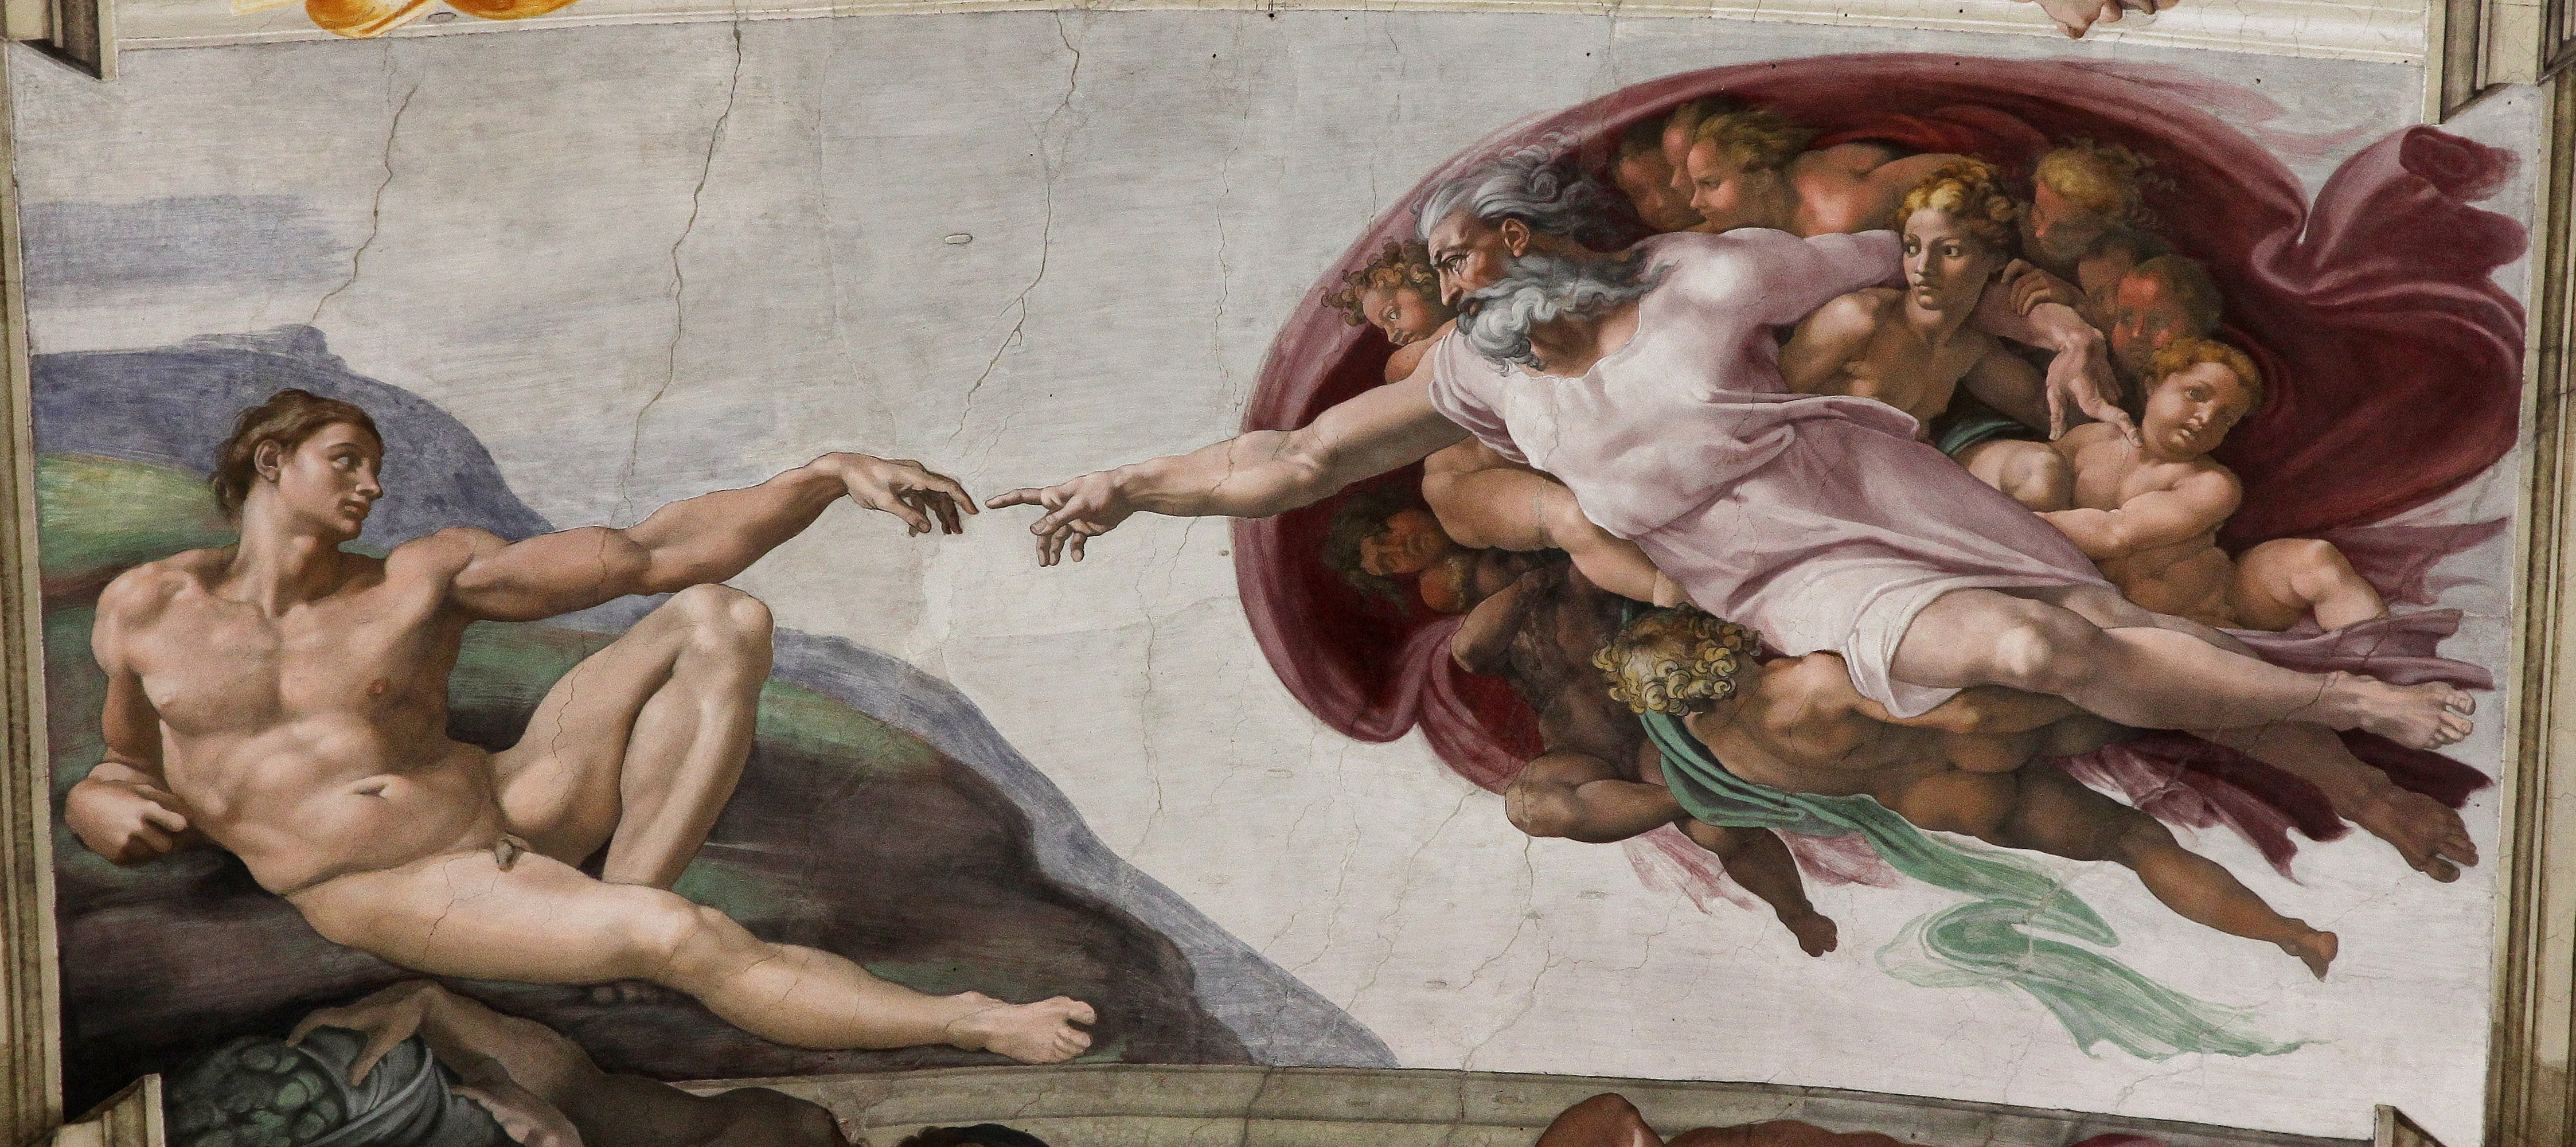
\includegraphics[width= \textwidth]{sistine_chapel.jpg}
\end{center}


\end{frame}


 \section{Rückenmark}
 
 
 \begin{frame}{Funktionen des Rückenmarks}
     
     \begin{itemize}
         \item 
         Umsetzung von Motorprogrammen 
         \item
         Ansteuerung von \(\alpha\)-Motoneuronen (Vorderhorn)
         \item
         Koordination synergistischer Effektorgruppen
         \item
         Integration somatosensorischer Information mit deszendierenden Beweungsprogrammen
         \item
         Aszendierende Trakte zu supraspinalen Zentren
         \item
         Reflexzentrum: Motorische Reflexe können unabhängig von supraspinalen Zentren durcheführt werden (werden aber durch diese moduliert)
         
     \end{itemize}
     
 \end{frame}
 
  \begin{frame}{Organisation des Rückenmarks}


\begin{columns}[c]

\begin{column}{5cm}
\begin{center}
    \includegraphics[width=\textwidth]{rueckenmark_orga.png}
\end{center}

\end{column}

\begin{column}{6cm}
Bewegungsanleitungen werden durch deszendierende Bahnen an spinale Neuronen weiter gegeben. \\[0.2 cm]
         
         
         Afferente Bahnen und deszendierende Motorefferenzen konvergieren i.d.R. auf spinalen Interneuronen. Dies erlaubt eine Modifikation des Bewegunsprogramms und Anpassung an tatsächliche Gegebenheiten. \\[0.2 cm]
         
         Aktualisierte Motorinstruktoin wird an \(\alpha\)-Motoneurone weitergeleitet, und es kommt schließlich zur Muskelkontraktion
\end{column}


\end{columns}


\end{frame}
 
  \section{Reflexe}

\begin{frame}{Reflexe: Grundlagen}
    
\textbf{Reflexweg}: Rezeptor \(\rightarrow\) Afferenz \(\rightarrow\) (ZNS-Verarbeitungsystem, z.B. spinale Interneuronen) \(\rightarrow\) Efferenz (\(\alpha\)-Motoneuronen) \(\rightarrow\) Muskel


\begin{center}
    \includegraphics[width=0.8\textwidth]{reflex_arc.png}
\end{center}

\end{frame}

\begin{frame}{Reflexe: Grundlagen}
 
 \begin{itemize}

     \item 
     \textbf{Reflexantwort}: abhängig von Reizstärke
     \begin{itemize}
     \item Amplitude (Je stärker der Reiz, desto größer der Reflex)
     \item Repertoire an Bewegungen (je nach Reizstärke können andere Körperteile miteinbezogen werden.)
     \end{itemize}
     Was sich \textbf{nicht} ändert ist die Latenz! \textcolor{theme}{Warum nicht?}  \pause \\
     Nur weil der Reiz stärker ist, wird die Reizleitung durch den Reflexweg nicht schneller
    
    \pause
    \item 
          \textbf{Eigenreflex}: Rezeptor und Effektor sind im selben Organ; kann monosynaptisch sein
\item     
          \textbf{Fremdreflex}: Rezeptor und Effektor sind in verschiedenen Organen; immer polysynaptisch
     
 \end{itemize}


\end{frame}

{ \usebackgroundtemplate{\includegraphics[width=1.0\paperwidth]{muskeldehnungsreflex.png}} 
\begin{frame}

 
\end{frame} 
}

{ \usebackgroundtemplate{\includegraphics[width=1.0\paperwidth]{muskeldehnungsreflex_2.png}} 
\begin{frame}

 
\end{frame} 
}


\begin{frame}{Rückwärtshemmung verhindert Überstimulierung von \(\alpha\)-Motoneuronen}

\begin{itemize}
    \item 
    Renshaw-Zellen sind glycinerge spinale Interneurone
    \item
    Die Renshaw-Zelle wird durch Kollaterale eines \(\alpha\)-Motoneuron stimuliert und inhibiert dann dieses \(\alpha\)-Motoneuron
    \item
    Diese Rückwärtshemmung verhindert zu hohe/zu lange Kontraktion des Muskels
    \item
    Supraspinale Zentren können Renshaw-Zellen inhibieren (und dadurch \(\alpha\)-Motoneuronen disinhibieren)
\end{itemize}   

\begin{center}
    \includegraphics[width=0.6\textwidth]{renshaw.png}
\end{center}

\end{frame}


\begin{frame}{Vorwärtshemmung dient der Spannungsstabilisierung im Muskel}


\begin{columns}[c]

\begin{column}{4cm}

\begin{center}
    \includegraphics[width=\textwidth]{vorwaertshemmung.png}
\end{center}

\end{column}

\begin{column}{7cm}
Verhindert das Afubauen von zu starker Spanning um Muskel \\[0.2 cm]
    Muskelspannung stimuliert 1b-Afferenz über Golgisehnenorgan \\[0.2 cm]
    1b Afferenz stimuliert hemmende (-) und erregende (+) Interneurone im Rückenmark \\[0.2 cm]
    Hemmende Interneurone hemmen \(\alpha\)-Motoneurone des Agonisten (Agonist hemmt sich selbst) \\[0.2 cm]
    Aktivierende Interneurone erregen \(\alpha\)-Motoneurone des \textbf{Anta}gonisten, der Antagonist kontrahiert \\[0.2 cm]
 
\end{column}


\end{columns}

\end{frame}
 
 
 \begin{frame}{H-Reflex}

\begin{itemize}
    \item 
    Experimentell (durch elektrische Stimulierung) ausgelöster Dehnungsreflex
    \item
    Reflexbogen: 1a-Faser, Axon \(\alpha\)-Motoneuron
    \item
    Antwort hängt von Reizstärke ab:

\end{itemize}

\begin{center}
    \includegraphics[width=\textwidth]{h_welle_m_welle.png}
\end{center}
     
     
     \pause
     

     Aber warum?
 \end{frame}
 
 
 %% h reflex niedrig mittel hoch
 
 %%%%%%%%%%%%%%%%%%%%%%%%%%%%%
 %%%%%%%%%%%%%%%%%%%%%%%%%%%%%
  %%%%%%%%%%%%%%%%%%%%%%%%%%%%%
 
 
%% VOR: Demo

%% VOR: Prinzip
\begin{frame}{Der vestibulo-okulärer Reflex koordiniert Augen- und Kopfbewegung}

\begin{center}
 \includegraphics[width=0.6\textwidth]{Simple_vestibulo-ocular_reflex.PNG}   
\end{center}
    
\end{frame} 
 
%% VOR: Differenzsignal

%% %% %% %% Review

\begin{frame}

 \frametitle{Jetzt* sollten Sie folgendes können}



\end{frame}




%% %% %% %% Feedbackhinweisblock

\begin{frame}
\frametitle{Danke für Ihr Feedback!}

\begin{columns}[c]

\begin{column}{6cm}
\begin{center}
 \includegraphics[width=\textwidth]{smilie_balloons.jpg}
\end{center}

\end{column}

\begin{column}{4cm}


\begin{center}
\includegraphics[width=\textwidth]{feedback_QR.png}
\end{center}
\end{column}


\end{columns}
\end{frame}




%% %% %% Bildnachweis
\begin{frame}
\frametitle{Bildnachweis}
\begin{tiny}

Teile dieser Vorlesung wurden übernommen von einer Vorlesung von Prof. Maike Glitsch, Medical School Hamburg, der wir an dieser Stelle herzlich danken. Wo nicht anders gekennzeichnet, stammen Abbildungen aus dieser Vorlesung.  


 
\begin{itemize}

\item
Aktivierung von DHP Rezeptoren und Freisetzung von Calcium aus dem SR. Daniel Walsh and Alan Sved, CC BY-SA 4.0 \url{https://creativecommons.org/licenses/by-sa/4.0}, via Wikimedia Commons

\item
Anatomie des Kleinhirns. Aus Liss, B., Kätzel, D. (2019). Kleinhirn. In: Brandes, R., Lang, F., Schmidt, R.F. (eds) Physiologie des Menschen. Springer-Lehrbuch. Springer, Berlin, Heidelberg. \url{https://doi.org/10.1007/978-3-662-56468-4_46}

\item
Aufbau der Skelettmuskulatur. Montage von Raul654. CC BY-SA 3.0, \url{https://commons.wikimedia.org/w/index.php?curid=73744}

\item
Erschaffung Adams (sixtinische Kapelle). Michelangelo. Foto Von Jörg Bittner Unna - Eigenes Werk, CC BY 3.0, \url{https://commons.wikimedia.org/w/index.php?curid=46496746}

\item
Golgi-Sehnenorgan. By Henry Vandyke Carter - Henry Gray (1918) Anatomy of the Human Body. Bartleby.com: Gray's Anatomy, Plate 938, Public Domain, \url{https://commons.wikimedia.org/w/index.php?curid=566884}


\item

Interaktion von Aktin und Myosin im Muskel.         Von Almut Hampl - via E-Mail, CC BY-SA 4.0, \url{https://commons.wikimedia.org/w/index.php?curid=107054691}

\item
Kind mit Bauklötzen. Photo by \href{https://unsplash.com/@markusspiske?utm_source=unsplash&utm_medium=referral&utm_content=creditCopyText}{Markus Spiske} on \href{https://unsplash.com/s/photos/fine-motor-skills?utm_source=unsplash&utm_medium=referral&utm_content=creditCopyText}{Unsplash}
  

\item
Labyrinth. Von Henry Vandyke Carter - Henry Gray (1918) Anatomy of the Human Body, Bartleby.com: Gray's Anatomy, Tafel 924, Gemeinfrei, \url{https://commons.wikimedia.org/w/index.php?curid=5918184}


%% all lectures
\item
Luftballons mit frohen und traurigen Smilies. Photo by \href{https://unsplash.com/@artbyhybrid?utm_source=unsplash&utm_medium=referral&utm_content=creditCopyText}{Hybrid} on \href{https://unsplash.com/s/photos/feedback?utm_source=unsplash&utm_medium=referral&utm_content=creditCopyText}{Unsplash}
%%%%%%%%%%%
\end{itemize}
\end{tiny}
\end{frame}


\begin{frame}
\frametitle{Bildnachweis}
\begin{tiny}
\begin{itemize}
    
\item
Motorische Endplatte. CC BY-SA 3.0, \url{https://commons.wikimedia.org/w/index.php?curid=305017}


\item
Muskelspindel. Modifiziert (Farben, Lesbarkeit, Verhalten bei Dehnung und Stauchung) nach folgender Vorlage: The original uploader was Hati at German Wikipedia., translated to English and converted to .svg by Sbmehta, CC BY 2.5  \url{https://creativecommons.org/licenses/by/2.5}, via Wikimedia Commons



\item
Reflexhammer. By Polarlys - Own work, CC BY-SA 4.0, \url{https://commons.wikimedia.org/w/index.php?curid=74272543}


\item
Reflexweg. By MartaAguayo - Own work, CC BY-SA 3.0, \url{https://commons.wikimedia.org/w/index.php?curid=39181552}

\item
Rückwärtshemmung durch Renshaw-Zelle. Aus: Frings, S., Müller, F. (2019). Die Sprache der Nervenzellen – und wie man sie versteht. In: Biologie der Sinne. Springer, Berlin, Heidelberg. \url{https://doi.org/10.1007/978-3-662-58350-0_3}

\item
Schichten de Zerebellums. Niels Chr. Danbolt, University of Oslo, Norway. via \url{https://neurotransporter.org/Cerebellum.html} Reproduction is permitted provided the author is acknowledged


\item
Spielzeug-Arztkoffer. Cristiano Betta on Flickr,  \url{https://www.flickr.com/photos/cristiano_betta/432834207}, CC-BY 2.0, 2007.

\item
Vestibulo-okulärer Reflex. By User:Mikael Häggström - Image:ThreeNeuronArc.pngOriginal uploader was Tvil at en.wikipedia, CC BY-SA 3.0, \url{https://commons.wikimedia.org/w/index.php?curid=2980751}

\end{itemize}
\end{tiny}
\end{frame}






\end{document}

%%% Frequently used snippets

%% \begin{columns}[c]

%% \begin{column}{5cm}
%% \end{column}

%% \begin{column}{5cm}
%% \end{column}


%% \end{columns}




